\documentclass[12pt]{article}
\usepackage{fullpage}
\usepackage{url}
\usepackage{amsmath}
\usepackage{amsfonts}
\usepackage{algorithm}
\usepackage{algorithmic}
\usepackage{graphicx}
\usepackage{hyperref}
\usepackage{color}
\usepackage{listings}
\usepackage{verbatim}
\usepackage{enumitem}
\usepackage[parfill]{parskip}

\newcommand{\xb}{\mathbf{x}}
\newcommand{\yb}{\mathbf{y}}
\newcommand{\wb}{\mathbf{w}}
\newcommand{\Xb}{\mathbf{X}}
\newcommand{\Yb}{\mathbf{Y}}
\newcommand{\tr}{^T}
\newcommand{\hb}{\mathbf{h}}
\newcommand{\Hb}{\mathbf{H}}

\newcommand{\cmt}[1]{{\footnotesize\textcolor{red}{#1}}}
\newcommand{\todo}[1]{\cmt{TO-DO: #1}}

\title{CS294-112 Deep Reinforcement Learning HW2}

\author{ Heri Zhao
}

\date{Fall 2018}

\usepackage{courier}
 
\definecolor{codegreen}{rgb}{0,0.6,0}
\definecolor{codegray}{rgb}{0.5,0.5,0.5}
\definecolor{codepurple}{rgb}{0.58,0,0.82}
\definecolor{backcolour}{rgb}{0.95,0.95,0.92}

\lstdefinestyle{mystyle}{
    backgroundcolor=\color{backcolour},   
    commentstyle=\color{codegreen},
    keywordstyle=\color{magenta},
    numberstyle=\tiny\color{codegray},
    stringstyle=\color{codepurple},
    basicstyle=\footnotesize\ttfamily,
    breakatwhitespace=false,         
    breaklines=true,                 
    captionpos=b,                    
    keepspaces=true,                 
    %numbers=left,                    
    numbersep=5pt,                  
    showspaces=false,                
    showstringspaces=false,
    showtabs=false,                  
    tabsize=2
}

\lstset{style=mystyle}

\begin{document}

\maketitle

\section*{Problem 1}
\begin{enumerate}[label=(\alph*)]
  \item For any $t$, we have
  \begin{align*}
    & \mathbb{E}_{\tau \sim p_\theta(\tau)} \left[ \nabla_\theta \log \pi_\theta(a_t|s_t) \left(b(s_t)\right)\right] \\
    &= \mathbb{E}_{p_\theta(s_t, a_t)} \mathbb{E}_{p_\theta(\tau / s_t, a_t | s_t, a_t)} \left[ \nabla_\theta \log \pi_\theta(a_t|s_t) \left(b(s_t)\right)\right] \\
    &= \mathbb{E}_{p_\theta(s_t, a_t)} \left[ \nabla_\theta \log \pi_\theta(a_t|s_t) \left(b(s_t)\right)\right] \\
    &= \mathbb{E}_{p_\theta(s_t)} \mathbb{E}_{p_\theta(a_t | s_t)} \left[ \nabla_\theta \log \pi_\theta(a_t|s_t) \left(b(s_t)\right)\right] \\
    &= \mathbb{E}_{p_\theta(s_t)} \left[b(s_t) \int_{a_t} p_\theta(a_t | s_t) \nabla_\theta \log \pi_\theta(a_t|s_t) d_{a_t} \right] \\
    &= \mathbb{E}_{p_\theta(s_t)} \left[b(s_t)\nabla_\theta \int_{a_t} \pi_\theta(a_t|s_t) d_{a_t} \right] \\
    &= \mathbb{E}_{p_\theta(s_t)} \left[b(s_t)\nabla_\theta 1 \right] \\
    &= 0
  \end{align*}
  Hence,
  $$
  \sum_{t=1}^T \mathbb{E}_{\tau \sim p_\theta(\tau)}\left[ \nabla_\theta \log \pi_\theta(a_t|s_t) \left(b(s_t)\right)\right] = 0
  $$

  \newpage
  \item Becasue it is MDP problem, so future states and actions of the process conditional on both past and present values, depends only upon the present state. Therefore,
  $$
  p_\theta(s_{t+1:T}, a_{t:T} | s_{1:t}, a_{1:t-1}) = p_\theta(s_{t+1:T}, a_{t:T} | s_t)
  $$
  Now we sow the equation 12:
  \begin{align*}
   & \mathbb{E}_{\tau \sim p_\theta(\tau)}\left[ \nabla_\theta \log \pi_\theta(a_t|s_t) \left(b(s_t)\right)\right] \\
    &= \mathbb{E}_{p_\theta(s_{1:t}, a_{1:t-1})} \mathbb{E}_{p_\theta(s_{t+1:T}, a_{t:T} | s_t)} \left[ \nabla_\theta \log \pi_\theta(a_t|s_t) \left(b(s_t)\right)\right] \\
    &= \mathbb{E}_{p_\theta(s_{1:t}, a_{1:t-1})} \mathbb{E}_{p_\theta(a_t | s_t)} \mathbb{E}_{p_\theta(s_{t+1:T}, a_{t:T} | s_t, a_t)} \left[ \nabla_\theta \log \pi_\theta(a_t|s_t) \left(b(s_t)\right)\right] \\
    &= \mathbb{E}_{p_\theta(s_{1:t}, a_{1:t-1})} \mathbb{E}_{p_\theta(a_t | s_t)} \left[ \nabla_\theta \log \pi_\theta(a_t|s_t) \left(b(s_t)\right)\right] \\
    &= \mathbb{E}_{p_\theta(s_{1:t}, a_{1:t-1})} \left[\int_{s_t} \int_{a_t} p_\theta(a_t | s_t) \nabla_\theta \log \pi_\theta(a_t|s_t) \left(b(s_t)\right)\right] \\
    &= \mathbb{E}_{p_\theta(s_{1:t}, a_{1:t-1})} \left[\int_{s_t} b(s_t) \nabla_\theta \int_{a_t} \pi_\theta(a_t|s_t) d_{a_t} d_{s_t} \right] \\
    &= \mathbb{E}_{p_\theta(s_{1:t}, a_{1:t-1})} \left[\int_{s_t} b(s_t) \nabla_\theta 1 \right] \\
    &= 0
  \end{align*}
  Hence,
  $$
  \sum_{t=1}^T \mathbb{E}_{\tau \sim p_\theta(\tau)}\left[ \nabla_\theta \log \pi_\theta(a_t|s_t) \left(b(s_t)\right)\right] = 0
  $$

\end{enumerate}

\newpage
\section*{Problem 4}
\begin{figure}[H]
  \centering
  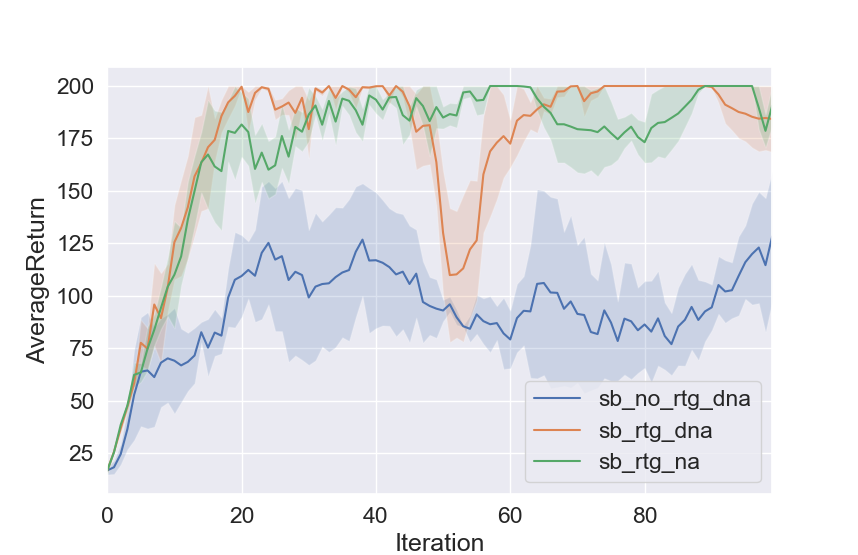
\includegraphics[height=3.4in]{p4_1.png}
  \caption{Learning curves for small batch experiments}
\end{figure}
\begin{lstlisting}[language=bash]
python train_pg_f18.py CartPole-v0 -n 100 -b 1000 -e 3 -dna --exp_name sb_no_rtg_dna
python train_pg_f18.py CartPole-v0 -n 100 -b 1000 -e 3 -rtg -dna --exp_name sb_rtg_dna
python train_pg_f18.py CartPole-v0 -n 100 -b 1000 -e 3 -rtg --exp_name sb_rtg_na
python plot.py data/sb_* --value AverageReturn
\end{lstlisting}

\begin{figure}[H]
  \centering
  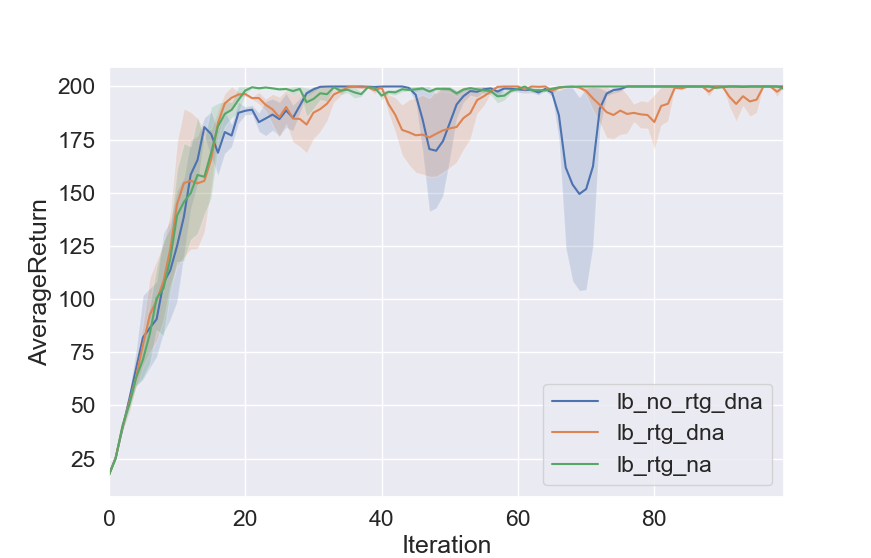
\includegraphics[height=3.3in]{p4_2.png}
  \caption{Learning curves for large batch experiments}
\end{figure}
\begin{lstlisting}[language=bash]
python train_pg_f18.py CartPole-v0 -n 100 -b 1000 -e 3 -dna --exp_name sb_no_rtg_dna
python train_pg_f18.py CartPole-v0 -n 100 -b 1000 -e 3 -rtg -dna --exp_name sb_rtg_dna
python train_pg_f18.py CartPole-v0 -n 100 -b 1000 -e 3 -rtg --exp_name sb_rtg_na
python plot.py data/lb_* --value AverageReturn
\end{lstlisting}
    
Answer the following questions briefly: 
  \begin{itemize}
  \item Which gradient estimator has better performance without advantage-centering---the trajectory-centric one, or the one using reward-to-go? \\
  \textbf{In small batch size case, we can see the one using reward-to-go gives higher average rewards and lower variance than the trajectory-centric one. In the large batch case, we can see there is not much difference on average rewards, but the variance is little better for reward-to-go one.}

  \item Did advantage centering help? \\
  \textbf{Advantage centering did help in terms of stabling the learning curve. In both small and large batch cases, though the green and orange curves have similar average rewards, the green curve is much more stable.}
  
  \item Did the batch size make an impact? \\
  \textbf{Yes, batch size did make an impact. It especially helped a lot for trajectory-centric and non-advantage-centering case (blue curve). It also helped the other two curve to converge to reward 200 faster.}
  \end{itemize}


\newpage
\section*{Problem 5}
$b* = 60, r* = 0.01$. The policy gets to stable at iteration about \#55.
\begin{figure}[H]
  \centering
  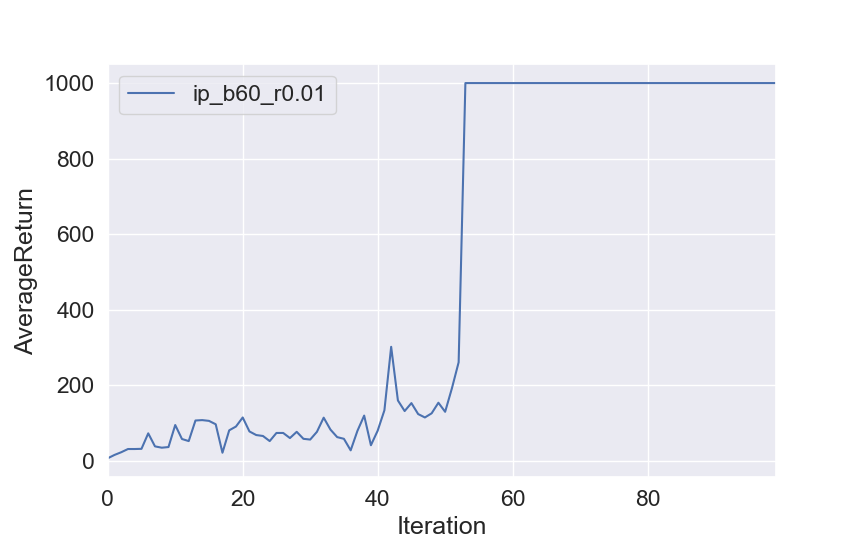
\includegraphics[height=3.5in]{p5.png}
  \caption{Learning Curve of InvertedPendulum with $b = 60$ and $lr = 0.01$ on specific $seed = 1$.}
\end{figure}
\begin{lstlisting}[language=bash]
python train_pg_f18.py InvertedPendulum-v2 -ep 1000 --discount 0.9 -n 100 -e 1 -l 2 -s 64 -b 60 -lr 0.01 -rtg --exp_name ip_b60_r0.01
python plot.py data/ip_b60_r0.01_InvertedPendulum-v2*
\end{lstlisting}


\newpage
\section*{Problem 7}
\begin{figure}[H]
  \centering
  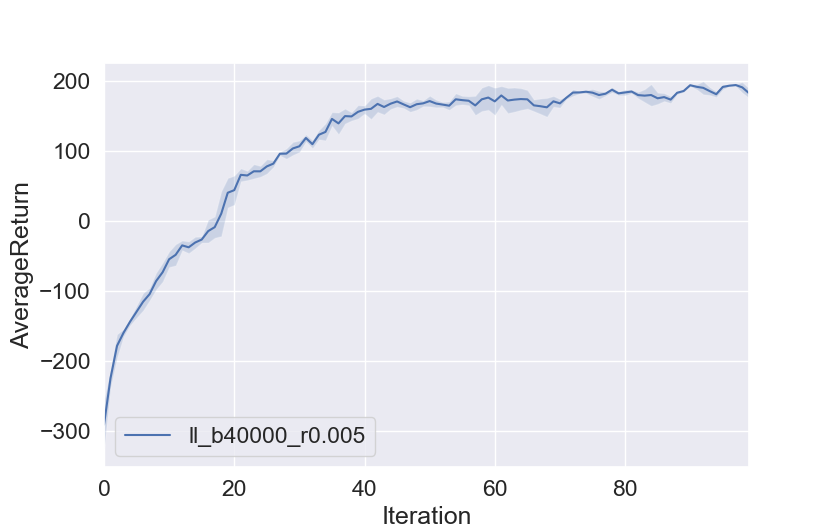
\includegraphics[height=3.5in]{p7.png}
  \caption{Learning Curve of LunarLander. The policy achieve an average return of around 180.}
\end{figure}
\begin{lstlisting}[language=bash]
python train_pg_f18.py LunarLanderContinuous-v2 -ep 1000 --discount 0.99 -n 100 -e 3 -l 2 -s 64 -b 40000 -lr 0.005 -rtg --nn_baseline --exp_name ll_b40000_r0.005
python plot.py data/ll_b40000_r0.005_LunarLanderContinuous-v2_* --value AverageReturn
\end{lstlisting}

\newpage
\section*{Problem 8}
\begin{figure}[H]
  \centering
  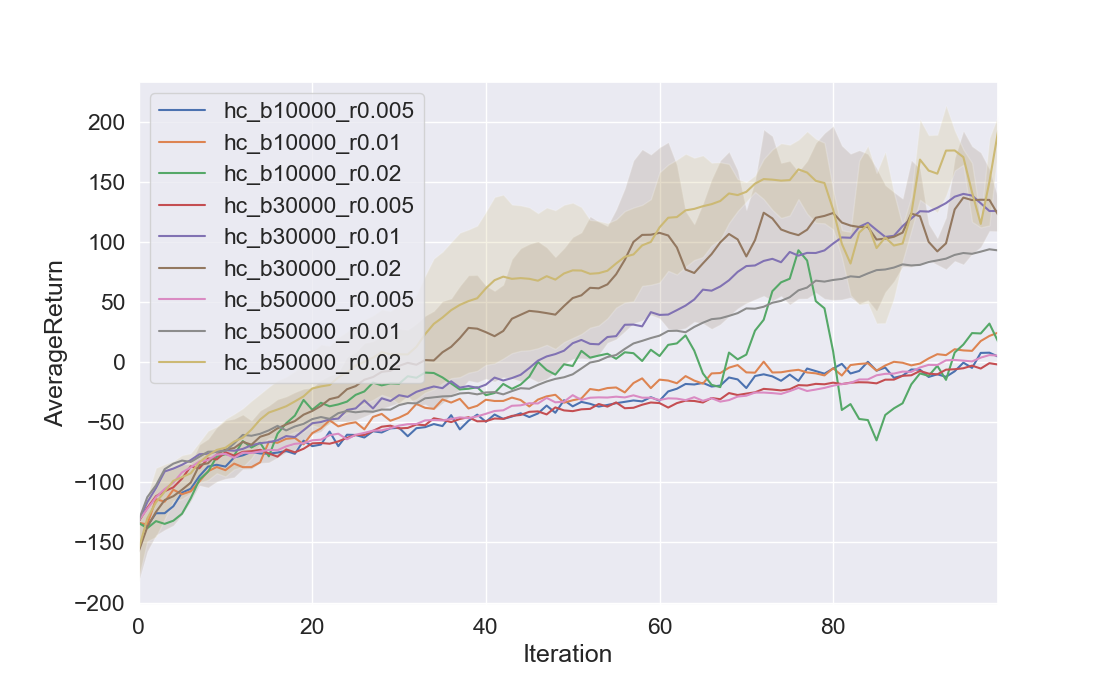
\includegraphics[height=4in]{p8_1.png}
  \caption{$3 \times 3$ hyper-parameter search. Best parameter is $b* = 50000$ and $r* = 0.02$}
\end{figure}
\begin{lstlisting}[language=bash]
python train_pg_f18.py HalfCheetah-v2 -ep 150 --discount 0.95 -n 100 -e 3 -l 2 -s 32 -b 10000 -lr 0.005 -rtg --nn_baseline --exp_name hc_b10000_r0.005
python train_pg_f18.py HalfCheetah-v2 -ep 150 --discount 0.95 -n 100 -e 3 -l 2 -s 32 -b 10000 -lr 0.01 -rtg --nn_baseline --exp_name hc_b10000_r0.01
python train_pg_f18.py HalfCheetah-v2 -ep 150 --discount 0.95 -n 100 -e 3 -l 2 -s 32 -b 10000 -lr 0.02 -rtg --nn_baseline --exp_name hc_b10000_r0.02
python train_pg_f18.py HalfCheetah-v2 -ep 150 --discount 0.95 -n 100 -e 3 -l 2 -s 32 -b 30000 -lr 0.005 -rtg --nn_baseline --exp_name hc_b30000_r0.005
python train_pg_f18.py HalfCheetah-v2 -ep 150 --discount 0.95 -n 100 -e 3 -l 2 -s 32 -b 30000 -lr 0.01 -rtg --nn_baseline --exp_name hc_b30000_r0.01
python train_pg_f18.py HalfCheetah-v2 -ep 150 --discount 0.95 -n 100 -e 3 -l 2 -s 32 -b 30000 -lr 0.02 -rtg --nn_baseline --exp_name hc_b30000_r0.02
python train_pg_f18.py HalfCheetah-v2 -ep 150 --discount 0.95 -n 100 -e 3 -l 2 -s 32 -b 50000 -lr 0.005 -rtg --nn_baseline --exp_name hc_b50000_r0.005
python train_pg_f18.py HalfCheetah-v2 -ep 150 --discount 0.95 -n 100 -e 3 -l 2 -s 32 -b 50000 -lr 0.01 -rtg --nn_baseline --exp_name hc_b50000_r0.01
python train_pg_f18.py HalfCheetah-v2 -ep 150 --discount 0.95 -n 100 -e 3 -l 2 -s 32 -b 50000 -lr 0.02 -rtg --nn_baseline --exp_name hc_b50000_r0.02
\end{lstlisting}
\begin{figure}[H]
  \centering
  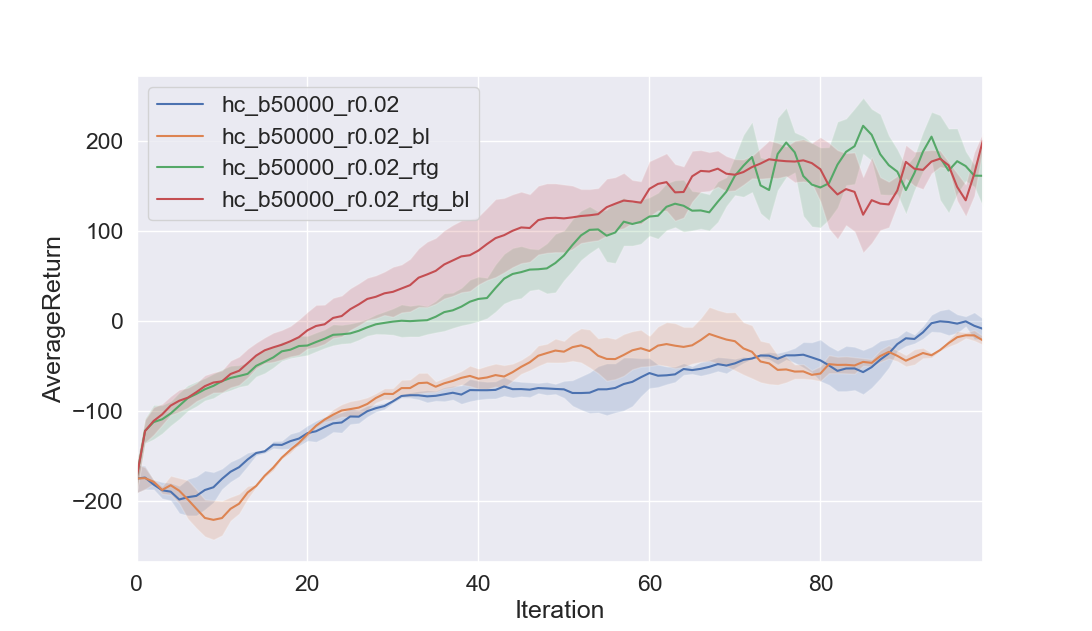
\includegraphics[height=4in]{p8_2.png}
  \caption{Learning Curve of HalfCheetah. The run with rtg and baseline achieves to reward around 200}
\end{figure}
\begin{lstlisting}[language=bash]
python train_pg_f18.py HalfCheetah-v2 -ep 150 --discount 0.95 -n 100 -e 3 -l 2 -s 32 -b 50000 -lr 0.02 --exp_name hc_b50000_r0.02
python train_pg_f18.py HalfCheetah-v2 -ep 150 --discount 0.95 -n 100 -e 3 -l 2 -s 32 -b 50000 -lr 0.02 -rtg --exp_name hc_b50000_r0.02_rtg
python train_pg_f18.py HalfCheetah-v2 -ep 150 --discount 0.95 -n 100 -e 3 -l 2 -s 32 -b 50000 -lr 0.02 --nn_baseline --exp_name hc_b50000_r0.02_bl
python train_pg_f18.py HalfCheetah-v2 -ep 150 --discount 0.95 -n 100 -e 3 -l 2 -s 32 -b 50000 -lr 0.02 -rtg --nn_baseline --exp_name hc_b50000_r0.02_rtg_bl
python plot.py data/hc_b50000_r0.02_*
\end{lstlisting}
How did the batch size and learning rate affect the performance? \\
\textbf{In this problem, larger batch size with same learning-rate will make learning/converging faster. For learning-rate, generally we need to pick a proper value so that it won't be too small or too large. Small learning-rate will help to stabilize the curve, but if it is too small, we have take more iterations to reach to the optimal, and there will be more chances being trapped by local minimum. Large learning-rate will help to increase convergence speed, but if it is too large, the curve will fluctuate a lot ending up with jumping from one local minimal to another instead of converging (e.g. green curve in Figure 5).}


\newpage
\section*{Bonus}
I implemented the GAE-$\lambda$, according to the following equations:
\begin{align*}
& A_t = \delta_t + \gamma \lambda A_{t+1} \\
& A_T = \delta_T = -V(s_T) + r_T + 0 \\
& \delta_t = -V(s_t) + r_t + \gamma V(s_{t+1})
\end{align*}
\begin{lstlisting}[language=python]
# Bonus part for GAE-lambda
adv_n = []
# A_t = delta_t + gamma * lambda * A_{t+1}
# A_T = delta_T = -V(s_T) + r_T + 0
# delta_t = -V(s_t) + r_t + gamma * V(s_{t+1})
index_b = 0
for re in re_n:
    adv_along_path = []
    last_v = 0  # V(s_{t+1})
    a_t = 0
    # we need to iterate the part of b_n corresponding to re in reversed order
    for r, v in zip(reversed(re), reversed(b_n[index_b: index_b + len(re)])):
        delta_t = -v + r + self.gamma * last_v
        a_t = delta_t + self.gamma * self.gae_lambda * a_t
        last_v = v
        adv_along_path.append(a_t)
    index_b += len(re)
    adv_along_path.reverse()
    adv_n.extend(adv_along_path)
# update q_n for fitting baseline later
q_n = b_n + adv_n
\end{lstlisting}
In Figure 7, we can see that the best $\lambda$ for GAE is 0.94 (red line). Compared with the case with default reward-to-go and baseline function (orange line, $\lambda=1$), GAE-$0.94$ is much more faster and achieves higher rewards at the end. \\
We can also notice that when $\lambda$ is too small or reach to $0$, the performance drops to even below non-value-function one (blue line).

\begin{figure}[H]
  \centering
  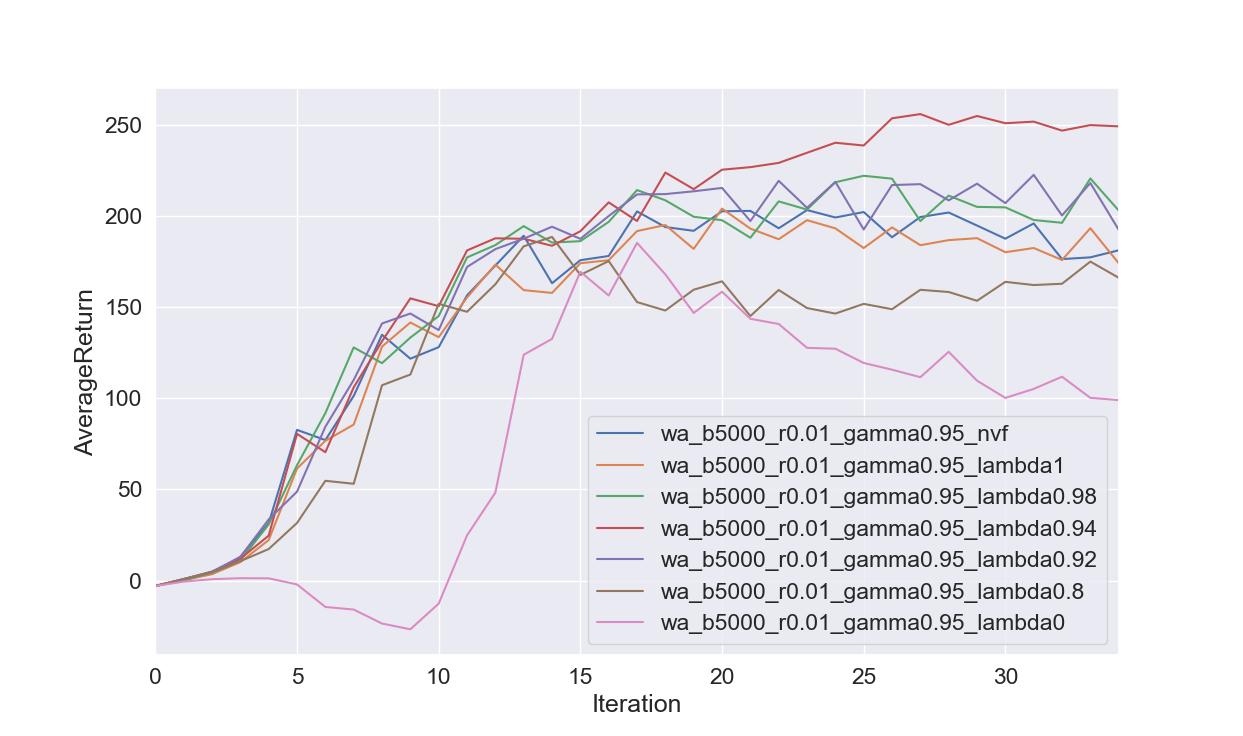
\includegraphics[height=4in]{bonus.png}
  \caption{Learning Curve for Walker2d-v2. Comparison of GAE-$\lambda$.}
\end{figure}
\begin{lstlisting}[language=bash]
python train_pg_f18.py Walker2d-v2 -ep 150 --discount 0.95 -n 35 -e 1 --seed 1 -l 2 -s 32 -b 5000 -lr 0.01 -rtg --exp_name wa_b5000_r0.01_gamma0.95_nvf
python train_pg_f18.py Walker2d-v2 -ep 150 --discount 0.95 -n 35 -e 1 --seed 1 -l 2 -s 32 -b 5000 -lr 0.01 -rtg --nn_baseline --exp_name wa_b5000_r0.01_gamma0.95_lambda1
python train_pg_f18.py Walker2d-v2 -ep 150 --discount 0.95 -n 35 -e 1 --seed 1 -l 2 -s 32 -b 5000 -lr 0.01 -rtg --nn_baseline --gae --gae_lambda 0.98 --exp_name  wa_b5000_r0.01_gamma0.95_lambda0.98
python train_pg_f18.py Walker2d-v2 -ep 150 --discount 0.95 -n 35 -e 1 --seed 1 -l 2 -s 32 -b 5000 -lr 0.01 -rtg --nn_baseline --gae --gae_lambda 0.94 --exp_name  wa_b5000_r0.01_gamma0.95_lambda0.94
python train_pg_f18.py Walker2d-v2 -ep 150 --discount 0.95 -n 35 -e 1 --seed 1 -l 2 -s 32 -b 5000 -lr 0.01 -rtg --nn_baseline --gae --gae_lambda 0.92 --exp_name  wa_b5000_r0.01_gamma0.95_lambda0.92
python train_pg_f18.py Walker2d-v2 -ep 150 --discount 0.95 -n 35 -e 1 --seed 1 -l 2 -s 32 -b 5000 -lr 0.01 -rtg --nn_baseline --gae --gae_lambda 0.8 --exp_name  wa_b5000_r0.01_gamma0.95_lambda0.8
python train_pg_f18.py Walker2d-v2 -ep 150 --discount 0.95 -n 35 -e 1 --seed 1 -l 2 -s 32 -b 5000 -lr 0.01 -rtg --nn_baseline --gae --gae_lambda 0 --exp_name  wa_b5000_r0.01_gamma0.95_lambda0
python plot.py data/wa_b5000_r0.01_gamma0.95*
\end{lstlisting}


\end{document}













